% Editable source for design.pdf: the frozen design of koblitz-n83-onlineframe-20261019 (from protocol.json; not a result).
\documentclass[tikz,border=6pt]{standalone}
\usepackage[T1]{fontenc}
\usetikzlibrary{positioning,arrows.meta}
\begin{document}
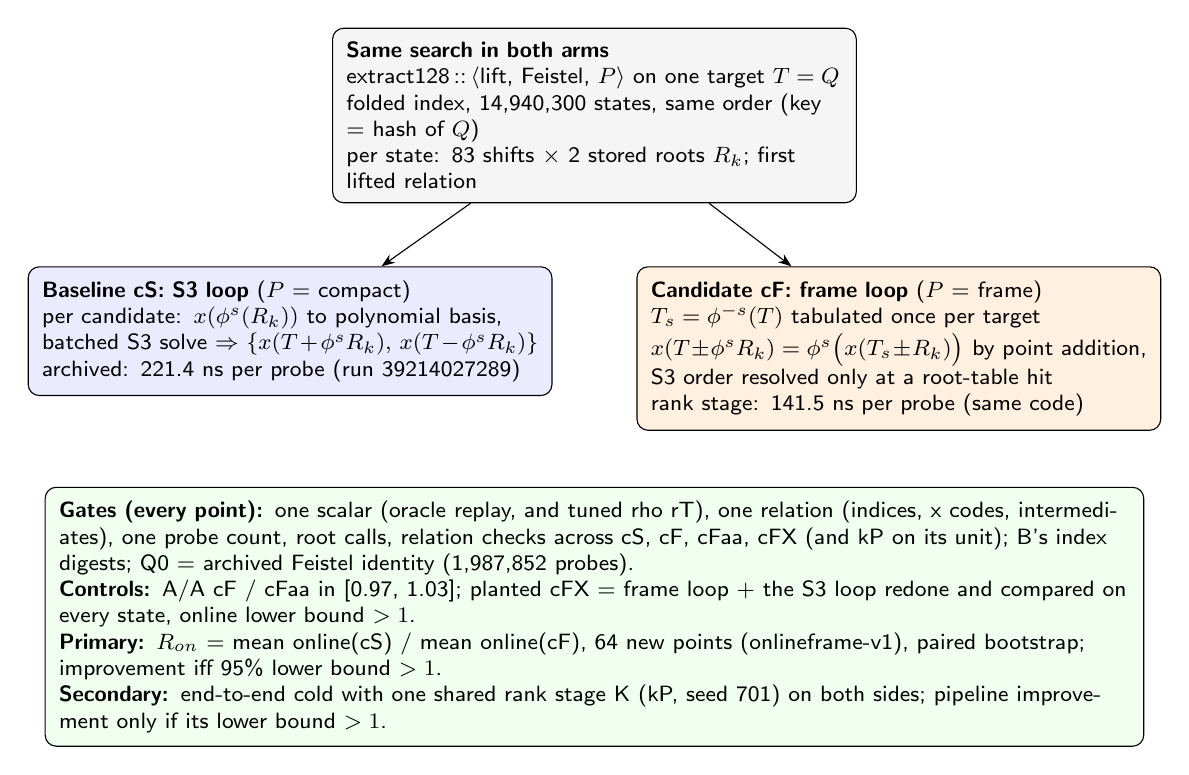
\begin{tikzpicture}[font=\sffamily\footnotesize, box/.style={draw,rounded corners,align=left,inner sep=5pt,text width=6.3cm},
  arm/.style={draw,rounded corners,align=left,inner sep=4pt,text width=4.1cm}, >=Stealth]
\node[box,fill=gray!8] (common) {\textbf{Same search in both arms}\\
extract128\,::\,$\langle$lift, Feistel, $P\rangle$ on one target $T=Q$\\
folded index, 14{,}940{,}300 states, same order (key = hash of $Q$)\\
per state: 83 shifts $\times$ 2 stored roots $R_k$; first lifted relation};
\node[box,fill=blue!8,below left=8mm and -28mm of common] (s3) {\textbf{Baseline cS: S3 loop} ($P$ = compact)\\
per candidate: $x(\phi^s(R_k))$ to polynomial basis,\\
batched S3 solve $\Rightarrow$ $\{x(T+\phi^sR_k),\,x(T-\phi^sR_k)\}$\\
archived: 221.4 ns per probe (run 39214027289)};
\node[box,fill=orange!12,below right=8mm and -28mm of common] (fr) {\textbf{Candidate cF: frame loop} ($P$ = frame)\\
$T_s=\phi^{-s}(T)$ tabulated once per target\\
$x(T\pm\phi^sR_k)=\phi^s\big(x(T_s\pm R_k)\big)$ by point addition,\\
S3 order resolved only at a root-table hit\\
rank stage: 141.5 ns per probe (same code)};
\draw[->] (common) -- (s3); \draw[->] (common) -- (fr);
\node[box,fill=green!6,below=36mm of common,text width=13.6cm] (gates) {\textbf{Gates (every point):} one scalar (oracle replay, and tuned rho rT), one relation (indices, x codes, intermediates), one probe count, root calls, relation checks across cS, cF, cFaa, cFX (and kP on its unit); B's index digests; Q0 = archived Feistel identity (1{,}987{,}852 probes).\\
\textbf{Controls:} A/A cF / cFaa in [0.97, 1.03]; planted cFX = frame loop + the S3 loop redone and compared on every state, online lower bound $>1$.\\
\textbf{Primary:} $R_{on}$ = mean online(cS) / mean online(cF), 64 new points (onlineframe-v1), paired bootstrap; improvement iff 95\% lower bound $>1$.\\
\textbf{Secondary:} end-to-end cold with one shared rank stage K (kP, seed 701) on both sides; pipeline improvement only if its lower bound $>1$.};
\end{tikzpicture}
\end{document}
